\documentclass[a4paper,12pt]{article}

\usepackage[utf8]{inputenc}
\usepackage[T1]{fontenc}
\usepackage{amsmath}
\usepackage{booktabs}
\usepackage{graphicx}
\usepackage{geometry}
\geometry{margin=2.5cm}
\usepackage{xcolor}
\usepackage{listings}
\usepackage{hyperref}
\hypersetup{colorlinks=true, linkcolor=blue!50!black, urlcolor=blue!50!black}
\renewcommand{\tablename}{Tabela}
\renewcommand{\lstlistingname}{Código}

% ---------- Configuração do realce de sintaxe (C) ----------
\definecolor{codebg}{RGB}{247,247,247}
\definecolor{codekw}{RGB}{0,0,180}
\definecolor{codecomment}{RGB}{0,128,0}
\definecolor{codestring}{RGB}{163,21,21}
\definecolor{framecolor}{RGB}{200,200,200}

\lstdefinestyle{cstyle}{
    language=C,
    backgroundcolor=\color{codebg},
    basicstyle=\ttfamily\footnotesize,
    keywordstyle=\color{codekw}\bfseries,
    commentstyle=\color{codecomment}\itshape,
    stringstyle=\color{codestring},
    numberstyle=\tiny\color{gray},
    numbers=left,
    numbersep=6pt,
    frame=single,
    rulecolor=\color{framecolor},
    breaklines=true,
    breakatwhitespace=false,
    showstringspaces=false,
    tabsize=4,
    captionpos=b,
    columns=flexible,
    morekeywords={size_t},
    extendedchars=true,
    literate=
        {á}{{\'a}}1 {à}{{\`a}}1 {â}{{\^a}}1 {ã}{{\~a}}1
        {é}{{\'e}}1 {ê}{{\^e}}1 {í}{{\'i}}1
        {ó}{{\'o}}1 {ô}{{\^o}}1 {õ}{{\~o}}1
        {ú}{{\'u}}1 {ü}{{\"u}}1 {ç}{{\c c}}1
        {Á}{{\'A}}1 {À}{{\`A}}1 {Â}{{\^A}}1 {Ã}{{\~A}}1
        {É}{{\'E}}1 {Ê}{{\^E}}1 {Í}{{\'I}}1
        {Ó}{{\'O}}1 {Ô}{{\^O}}1 {Õ}{{\~O}}1
        {Ú}{{\'U}}1 {Ü}{{\"U}}1 {Ç}{{\c C}}1
}

\title{Contagem de Números Primos com OpenMP: Sequencial vs. Paralelo}
\author{Israel Soares de Castro Filho \\ Matrícula: 20250070780}
\date{}

\begin{document}

\maketitle

\section{Introdução}

Este relatório apresenta a implementação e a avaliação experimental de um programa em C
que conta a quantidade de números primos existentes no intervalo $[2, n]$, comparando uma
versão sequencial com uma versão paralelizada por meio da diretiva \texttt{\#pragma omp
parallel for} da biblioteca OpenMP. O objetivo é observar o ganho de desempenho obtido com
a paralelização, bem como identificar e discutir problemas de correção que podem surgir
quando múltiplas threads acessam e modificam uma mesma variável compartilhada sem qualquer
mecanismo de sincronização — no caso, a variável de contagem \texttt{contagem\_par}.

\section{Metodologia}

O programa recebe uma lista de valores de $n$ ($1.000.000$, $5.000.000$, $10.000.000$,
$15.000.000$ e $20.000.000$) e, para cada um deles, executa duas versões do mesmo
algoritmo de contagem de primos:

\begin{itemize}
    \item \textbf{Versão sequencial}: percorre o intervalo $[2, n]$ em um único laço
    \texttt{for}, testando a primalidade de cada número com a função
    \texttt{verificar\_primo} (teste de divisibilidade por tentativa até $\sqrt{num}$) e
    incrementando a variável \texttt{contagem\_seq}.
    \item \textbf{Versão paralela}: executa exatamente o mesmo laço, porém precedido pela
    diretiva \texttt{\#pragma omp parallel for}, que distribui as iterações entre as
    threads disponíveis. O incremento é feito na variável compartilhada
    \texttt{contagem\_par}, sem uso de \texttt{reduction}, \texttt{atomic} ou
    \texttt{critical}.
\end{itemize}

O tempo de execução de cada versão foi medido com \texttt{omp\_get\_wtime()}. Os testes
foram executados em uma máquina com 8 núcleos disponíveis (\texttt{omp\_get\_num\_procs()
= 8}). O código-fonte completo encontra-se no Apêndice~\ref{sec:codigo}.

\section{Resultados}

A Tabela~\ref{tab:resultados} resume a quantidade de primos encontrados, os tempos de
execução e a diferença entre as contagens sequencial e paralela para cada valor de $n$
testado.

\begin{table}[h!]
\centering
\caption{Resultados obtidos para cada valor de $n$ (8 núcleos disponíveis).}
\label{tab:resultados}
\begin{tabular}{@{}rrrrrr@{}}
\toprule
$n$ & Primos (Seq.) & Primos (Par.) & Tempo Seq. (s) & Tempo Par. (s) & Diferença \\
\midrule
1.000.000  & 78.498    & 76.652    & 0,3710  & 0,1140 & 1.846 \\
5.000.000  & 348.513   & 344.713   & 3,6930  & 1,0480 & 3.800 \\
10.000.000 & 664.579   & 659.197   & 9,8250  & 2,8370 & 5.382 \\
15.000.000 & 970.704   & 963.832   & 17,5090 & 4,8950 & 6.872 \\
20.000.000 & 1.270.607 & 1.262.967 & 26,4810 & 7,4820 & 7.640 \\
\bottomrule
\end{tabular}
\end{table}

A Tabela~\ref{tab:speedup} apresenta o \textit{speedup} (razão entre o tempo sequencial e
o tempo paralelo), a eficiência (speedup dividido pelo número de núcleos) e o erro
percentual da contagem paralela em relação à contagem sequencial (considerada correta).

\begin{table}[h!]
\centering
\caption{Speedup, eficiência e erro percentual da contagem.}
\label{tab:speedup}
\begin{tabular}{@{}rrrr@{}}
\toprule
$n$ & Speedup & Eficiência (\%) & Erro na contagem (\%) \\
\midrule
1.000.000  & 3,25 & 40,7 & 2,35 \\
5.000.000  & 3,52 & 44,1 & 1,09 \\
10.000.000 & 3,46 & 43,3 & 0,81 \\
15.000.000 & 3,58 & 44,7 & 0,71 \\
20.000.000 & 3,54 & 44,2 & 0,60 \\
\bottomrule
\end{tabular}
\end{table}

A Figura~\ref{fig:grafico} ilustra a evolução do tempo de execução das duas versões e do
speedup obtido em função do tamanho do intervalo $n$.

\begin{figure}[h!]
\centering
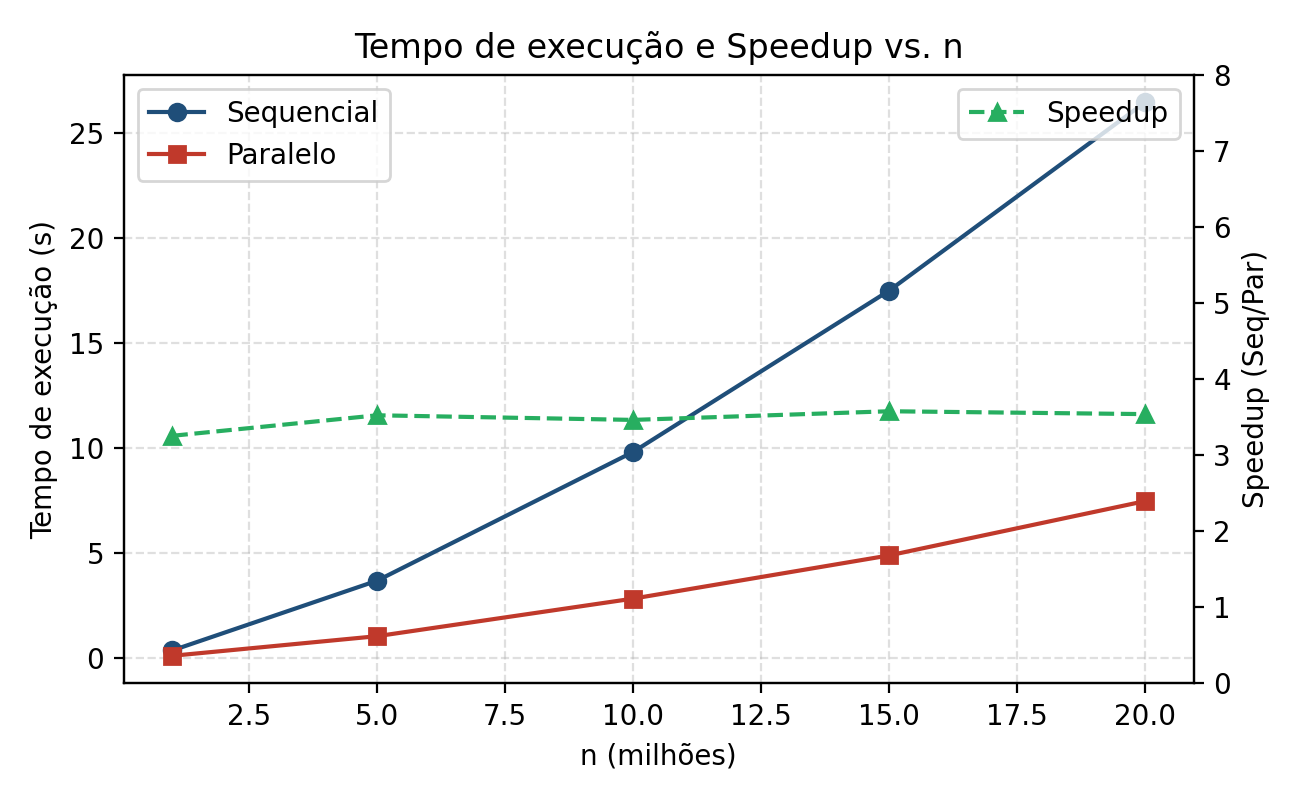
\includegraphics[width=0.85\textwidth]{images/grafico_desempenho.png}
\caption{Tempo de execução (sequencial e paralelo) e speedup em função de $n$.}
\label{fig:grafico}
\end{figure}

Em todos os cinco casos testados, a versão paralela apresentou um número de primos
\textbf{menor} do que a versão sequencial, e a mensagem \texttt{[ALERTA] Os resultados
divergem!} foi disparada em 100\% das execuções.

\section{Análise}

\subsection{Desempenho}

O tempo de execução da versão sequencial cresce de forma aproximadamente proporcional a
$n$ (na verdade, um pouco mais que linear, já que o custo do teste de primalidade de cada
número cresce com $\sqrt{num}$). A versão paralela acompanha essa mesma tendência de
crescimento, porém com um tempo consistentemente menor. O speedup obtido variou entre
$3{,}25\times$ e $3{,}58\times$, estabilizando-se em torno de $3{,}5\times$ para os
valores de $n$ maiores. Como a máquina possui 8 núcleos disponíveis, o speedup ideal
(linear) seria próximo de $8\times$; o valor observado corresponde a uma eficiência de
apenas $\sim$41--45\%.

Esse distanciamento do speedup ideal é esperado nesta implementação simples e pode ser
atribuído a:

\begin{itemize}
    \item \textbf{Desbalanceamento de carga}: o \texttt{\#pragma omp parallel for} sem uma
    cláusula \texttt{schedule} explícita usa, por padrão, a política \texttt{static},
    dividindo o intervalo $[2, n]$ em blocos contíguos de tamanho igual entre as threads.
    
    Como o custo de \texttt{verificar\_primo(num)} cresce com $\sqrt{num}$, threads
    responsáveis pelas faixas de números maiores realizam mais trabalho do que as
    responsáveis pelas faixas iniciais, gerando desbalanceamento de carga.
    
    \item \textbf{Condição de corrida no incremento de \texttt{contagem\_par}}: sem
    \texttt{reduction}, \texttt{atomic} ou \texttt{critical}, múltiplas threads leem,
    incrementam e escrevem a mesma variável compartilhada concorrentemente, o que também
    poder ter um efeito (secundário) na parte de custo do sincronismo implícito de cache
    (falso compartilhamento / \textit{cache invalidation}), embora o principal efeito
    observado aqui seja sobre a \emph{correção}, discutido a seguir.
    
    \item \textbf{Overhead de criação e sincronização das threads}, que se torna
    proporcionalmente menor à medida que $n$ aumenta — o que explica por que o speedup
    tende a estabilizar (e até melhorar ligeiramente) para os valores maiores de $n$.
\end{itemize}

\subsection{Correção: a condição de corrida}

O resultado mais importante desta atividade não é o ganho de desempenho, mas o problema de
\textbf{correção} evidenciado em \emph{todas} as execuções: a contagem paralela foi sempre
\textbf{menor} do que a sequencial, nunca maior e nunca igual.

Isso ocorre porque a operação \texttt{contagem\_par++} não é atômica. Internamente, ela
corresponde a três passos: (1) ler o valor atual de \texttt{contagem\_par}, (2) somar 1,
e (3) escrever o novo valor de volta na memória. Quando duas ou mais threads executam
esses três passos de forma intercalada sobre a mesma variável, é possível que ambas leiam
o mesmo valor antes que qualquer uma escreva o resultado incrementado; nesse caso, um dos
incrementos é ``perdido''. Como esse tipo de sobreposição depende do escalonamento das
threads pelo sistema operacional, o resultado final é nao determinístico — porém, com um
número suficientemente grande de primos a contar (e, portanto, de incrementos disputados),
a tendência estatística é sempre de \emph{perda} de incrementos, nunca de excesso, o que
explica por que a contagem paralela é sistematicamente menor.

\subsection{Reflexão sobre os desafios da programação paralela}

Este experimento evidencia dois desafios centrais e complementares no início da
programação paralela:

\begin{enumerate}
    \item \textbf{Correção antes de desempenho}: paralelizar um laço sem analisar as
    dependências entre iterações (neste caso, a dependência de todas as iterações sobre a
    mesma variável \texttt{contagem\_par}) produz um programa mais rápido, porém incorreto.
    Um ganho de desempenho não tem valor se o resultado produzido não é confiável. A
    correção deveria ser restaurada, por exemplo, substituindo a diretiva por
    \texttt{\#pragma omp parallel for reduction(+:contagem\_par)}, que garante que cada
    thread mantenha uma cópia local do acumulador e that as combine de forma segura ao
    final, sem custo de sincronização a cada iteração.
    \item \textbf{Distribuição de carga}: mesmo corrigindo a condição de corrida, o
    desbalanceamento causado pelo custo não uniforme de \texttt{verificar\_primo} continuaria
    limitando o speedup máximo alcançável com um escalonamento puramente estático. Nesse
    caso, testar cláusulas como \texttt{schedule(dynamic)} ou \texttt{schedule(guided)}
    tenderia a melhorar a distribuição de trabalho entre as threads, aproximando o speedup
    obtido do speedup teórico permitido pelo número de núcleos.
\end{enumerate}

\section{Conclusão}

A paralelização do laço de contagem de primos com OpenMP produziu um speedup médio de
aproximadamente $3{,}5\times$ em uma máquina com 8 núcleos, evidenciando ganho real de
desempenho, mas distante do ideal devido ao desbalanceamento de carga inerente ao
escalonamento estático padrão. Mais relevante do que o ganho de tempo, porém, foi a
demonstração prática de que paralelizar um laço "sem alterar a lógica original" não é
suficiente para garantir resultados corretos: a ausência de sincronização no incremento de
uma variável compartilhada gerou uma condição de corrida que subestimou sistematicamente a
contagem de primos em todos os cinco cenários testados, com erro absoluto crescente e erro
relativo decrescente à medida que $n$ aumentava. O experimento reforça que, na programação
paralela, a verificação de corretude (por meio de mecanismos como \texttt{reduction},
\texttt{atomic} ou \texttt{critical}) deve caminhar lado a lado com a busca por desempenho,
e que a distribuição desigual de trabalho entre threads é um segundo aspecto que também
precisa ser avaliado e ajustado (por exemplo, com diferentes políticas de
\texttt{schedule}) para que o potencial de paralelismo do hardware seja de fato aproveitado.

\newpage
\appendix

\section{Código-Fonte}
\label{sec:codigo}

O código-fonte completo utilizado nos testes está disponível em
\texttt{../src/tarefa5.c} e é reproduzido a seguir.

\lstinputlisting[style=cstyle, caption={Contagem de primos sequencial e paralela (OpenMP).}]{../src/tarefa5.c}

\end{document}